其中最后一步把剩余的所有张量收缩并合并为最终的核心张量 $\Gt_4$。可以证明，这一流程与执行 TT-SVD \emph{完全}等价。

如人所料，本章并未涵盖其他一些张量网络。下一节简要介绍其中几种，它们都是 Tucker 分解与 TT 分解的重要推广。
\subsection{其他分解：张量环、投影纠缠对态（PEPS）\& 层次 Tucker}

张量列（TT）的一种常见推广是张量环（Tensor Ring, TR）分解。
\paragraph{张量环分解}
张量环分解是 TT 分解的推广~\citep{zhao2016tensor}。它最初出现于量子物理，近年来在机器学习社区中逐渐流行起来~\citep{wang2017efficient,wang2018wide,yuan2018higher}。尽管 TR 分解存在若干数值稳定性方面的问题~\citep{batselier2018trouble,chen2020tensor}，实践中它一般所需参数更少，压缩率也高于 TT 分解~\citep{mickelin2020algorithms}。设 $\Xt\in\RR^{d_1\times\dots\times d_N}$
    为 $N$ 阶张量。再设
    $\Gt_n\in\RR^{R_{n-1}\times d_n\times R_n}$（$n\in[N]$）为核心张量。
    张量 $\Xt$ 的秩 $R$ 的\emph{张量环分解}由下式给出
\begin{align*}
    \Xt_{i_1,\dots,i_N}=\hspace{0.25cm}\sum_{r_1=1}^{R_1}\dots\sum_{r_{N}=1}^{R_N}
    (\Gt_1)_{r_N,i_1,r_1} (\Gt_2)_{ r_1,i_2,r_2}\dots  (\Gt_{N-1})_{r_{N-2},i_{N-1},r_{N-1}} (\Gt_{N})_{r_{N-1},i_{N},r_N},
\end{align*}
对所有指标 $i_1\in[d_1],\cdots,i_N\in[d_N]$ 均成立。
四阶张量的 TR 分解可用张量网络记法表示如下：
$$
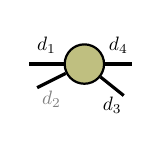
\begin{tikzpicture}[baseline=-0.5ex]
    \tikzset{tensor/.style = {minimum size = 0.5cm,shape = circle,thick,draw=black,inner sep = 0pt}, edge/.style = {thick,line width=.4mm},every loop/.style={}}
    \def\x{6}
    \def\y{0}
     \node[tensor,fill=green!50!red!50!white] (B) at (\x+1,\y) {$\Xt$};
    \draw[edge] (B) -- (\x+0.3,0) node [midway,above] {\scalebox{0.7}{\dimcolor{$d_1$}}};
    \draw[edge] (B) -- (\x+1.6,0) node [midway,above] {\scalebox{0.7}{\dimcolor{$d_4$}}};;
    \draw[edge] (B) -- (\x+0.4,-0.3) node [midway, below] {\scalebox{0.7}{\textcolor{gray}{$d_2$}}};;
    \draw[edge] (B) -- (\x+1.5,-0.4)node [midway, below] {\scalebox{0.7}{\dimcolor{$d_3$}}};;
\end{tikzpicture}=
\begin{tikzpicture}[baseline=\baseline]
    \tikzset{tensor/.style = {minimum size = 0.5cm,shape = circle,thick,draw=black,inner sep = 0pt}, edge/.style   = {thick,line width=.4mm},every loop/.style={}}
    \def\y{0}
    \def\x{0}
  \node[tensor,fill=red!30!white] (D) at (\x-1,\y){$\Gt_1$};
  \node[tensor,fill=red!50!white] (A) at (\x,\y){$\Gt_2$};
  \node[tensor,fill=blue!50!white] (B) at (\x+1,\y){$\Gt_3$};
   \node[tensor,fill=blue!20!white] (C) at (\x+2,\y){$\Gt_4$};
    \draw[edge](A) -- (\x,\y-0.7)node [midway,left] {\edgelabel{$d_2$}};
    \draw[edge](B) -- (\x+1,\y-0.7)node [midway,left] {\edgelabel{$d_3$}};
    \draw[edge](C) -- (\x+2,\y-0.7)node [midway,left] {\edgelabel{$d_4$}};
     \draw[edge](D) -- (\x-1,\y-0.7)node [midway,left] {\edgelabel{$d_1$}};
    \draw[edge](D) -- (A) node [midway,above] {\edgelabel{$R$}};
    \draw[edge](A) -- (B) node [midway,above] {\edgelabel{$R$}};
    \draw[edge](B) -- (C) node [midway,above] {\edgelabel{$R$}};
    \draw[edge] (D) to [out=145,in=35, distance=1cm] (C);
     \node[draw=none] () at (\x+0.5,\y+0.8) {\scalebox{0.7}{\dimcolor{$R$}}};
\end{tikzpicture}.
$$
作为张量环分解的特例，令所有秩都等于 1，便可得到一个秩一分解：
$$
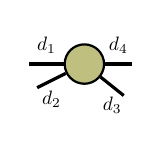
\begin{tikzpicture}[baseline=-0.5ex]
    \tikzset{tensor/.style = {minimum size = 0.5cm,shape = circle,thick,draw=black,inner sep = 0pt}, edge/.style = {thick,line width=.4mm},every loop/.style={}}
    \def\x{6}
    \def\y{0}
     \node[tensor,fill=green!50!red!50!white] (B) at (\x+1,\y) {$\Xt$};
    \draw[edge] (B) -- (\x+0.3,0) node [midway,above] {\scalebox{0.7}{\dimcolor{$d_1$}}};
    \draw[edge] (B) -- (\x+1.6,0) node [midway,above] {\scalebox{0.7}{\dimcolor{$d_4$}}};
    \draw[edge] (B) -- (\x+0.4,-0.3) node [midway, below] {\scalebox{0.7}{\dimcolor{$d_2$}}};
    \draw[edge] (B) -- (\x+1.5,-0.4)node [midway, below] {\scalebox{0.7}{\dimcolor{$d_3$}}};
\end{tikzpicture}=
\begin{tikzpicture}[baseline=\baseline]
    \tikzset{tensor/.style = {minimum size = 0.5cm,shape = circle,thick,draw=black,inner sep = 0pt}, edge/.style   = {thick,line width=.4mm},every loop/.style={}}
    \def\y{0}
    \def\x{0}
  \node[tensor,fill=red!30!white] (D) at (\x-1,\y){$\gb_1$};
  \node[tensor,fill=red!50!white] (A) at (\x,\y){$\gb_2$};
  \node[tensor,fill=blue!50!white] (B) at (\x+1,\y){$\gb_3$};
   \node[tensor,fill=blue!20!white] (C) at (\x+2,\y){$\gb_4$};
    \draw[edge](A) -- (\x,\y-0.7)node [midway,left] {\edgelabel{$d_2$}};
    \draw[edge](B) -- (\x+1,\y-0.7)node [midway,left] {\edgelabel{$d_3$}};
    \draw[edge](C) -- (\x+2,\y-0.7)node [midway,left] {\edgelabel{$d_4$}};
     \draw[edge](D) -- (\x-1,\y-0.7)node [midway,left] {\edgelabel{$d_1$}};
\end{tikzpicture}
=
\xb^1\outprod\xb^2\outprod\xb^3\outprod\xb^4.
$$
\paragraph{投影纠缠对态（PEPS）}
投影纠缠对态~（PEPS）一族由此成为把 TT 分解推广到量子物理中高阶格点结构的代表之一~\citep{verstraete2004renormalization,orus2014practical}。
PEPS 是由五阶核心张量按二维阵列排布而成的张量网络。对应于 $4\times 4$ 方格子的 PEPS 张量图如下：
$$
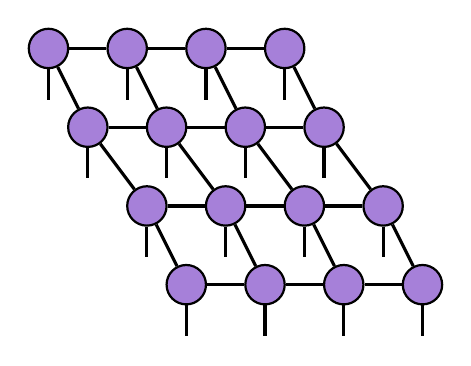
\begin{tikzpicture}[baseline=-0.5ex]
    \tikzset{tensor/.style = {minimum size = 0.5cm,shape = circle,thick,draw=black,inner sep = 0pt}, edge/.style = {thick,line width=.4mm},every loop/.style={}}
    \def\x{6}
    \def\y{0}
     \node[tensor,fill=red!30!blue!50!white] (A) at (\x,\y) {};
     \node[tensor,fill=red!30!blue!50!white] (B) at (\x+1,\y) {};
     \node[tensor,fill=red!30!blue!50!white] (C) at (\x+2,\y) {};
     \node[tensor,fill=red!30!blue!50!white] (D) at (\x+0.5,\y-1) {};
     \node[tensor,fill=red!30!blue!50!white] (E) at (\x+1.5,\y-1) {};
     \node[tensor,fill=red!30!blue!50!white] (F) at (\x+2.5,\y-1) {};
     \node[tensor,fill=red!30!blue!50!white] (G) at (\x+1.25,\y-2) {};
     \node[tensor,fill=red!30!blue!50!white] (H) at (\x+2.25,\y-2) {};
    \node[tensor,fill=red!30!blue!50!white] (I) at (\x+3.25,\y-2) {};
     \node[tensor,fill=red!30!blue!50!white] (J) at (\x+3,\y) {};
     \node[tensor,fill=red!30!blue!50!white] (K) at (\x+3.5,\y-1) {};
     \node[tensor,fill=red!30!blue!50!white] (L) at (\x+4.25,\y-2) {};
     \node[tensor,fill=red!30!blue!50!white] (M) at (\x+1.75,\y-3) {};

     \node[tensor,fill=red!30!blue!50!white] (N) at (\x+2.75,\y-3) {};
     \node[tensor,fill=red!30!blue!50!white] (O) at (\x+3.75,\y-3) {};
     \node[tensor,fill=red!30!blue!50!white] (P) at (\x+4.75,\y-3) {};
     
     \draw[edge](A) --(B);
    \draw[edge](A) --(\x,\y-0.65);
    \draw[edge](A) --(D);
    \draw[edge](B) --(C);
    \draw[edge](B) --(\x+1,\y-0.65);
    \draw[edge](B) --(E);
    \draw[edge](D) --(E);
    \draw[edge](C) --(F);
    \draw[edge](C) -- (\x+2,\y-0.65);
    \draw[edge](E) --(F);
    \draw[edge](F) -- (\x+2.5,\y-1.65);
    \draw[edge](D) --(G);
    \draw[edge](D) -- (\x+0.5,\y-1.65);
    \draw[edge](G) --(H);
    \draw[edge](E) --(H);
    \draw[edge](E) -- (\x+1.5,\y-1.65);
    \draw[edge](H) --(I);
    \draw[edge](F) --(I);
    \draw[edge](G) -- (\x+1.25,\y-2.65);
    \draw[edge](H) -- (\x+2.25,\y-2.65);
    \draw[edge](I) -- (\x+3.25,\y-2.65);
    \draw[edge](C)--(J);
     \draw[edge](K)--(F);
    \draw[edge](I)--(L);
    \draw[edge](J)--(K);
    \draw[edge](K)--(L);
    \draw[edge](J) -- (\x+3,\y-0.65);
    \draw[edge](K) -- (\x+3.5,\y-1.65);
    \draw[edge](L) -- (\x+4.25,\y-2.65);
    \draw[edge](M)--(N);
    \draw[edge](N)--(O);
    \draw[edge](O)--(P);
    \draw[edge](G)--(M);
    \draw[edge](H)--(N);
    \draw[edge](I)--(O);
    \draw[edge](L)--(P);
    \draw[edge](M)--(\x+1.75,\y-3.65);
    \draw[edge](N)--(\x+2.75,\y-3.65);
    \draw[edge](O)--(\x+3.75,\y-3.65);
    \draw[edge](P)--(\x+4.75,\y-3.65);
\end{tikzpicture}
$$
\paragraph{树形张量网络/~层次 Tucker 分解}
另一种颇受关注的张量网络是树形张量网络~（Tree Tensor Networks, TTN）或层次 Tucker~（Hierarchical Tucker, HT）分解，最早见于~\citep{hackbusch2009new, grasedyck2010hierarchical}。这一张量网络的关键优势在于，与 TT 分解这类较简单的模型相比，它的表达能力更强。四阶张量的 HT 分解可用张量网络图表示如下：
$$
\begin{tikzpicture}[baseline=\baseline]
    \tikzset{tensor/.style = {minimum size = 0.5cm,shape = circle,thick,draw=black,inner sep = 0pt}, edge/.style   = {thick,line width=.4mm},every loop/.style={}}
    \def\y{0}
    \def\x{0}
    \node[tensor,fill=blue!30!red!50!white] (A) at (\x+0.5,\y+1) {};
    \node[tensor,fill=blue!30!red!50!white] (B) at (\x,\y) {};
  \node[tensor,fill=blue!30!red!50!white] (C) at (\x+1,\y){};
   \node[tensor,fill=blue!30!red!50!white] (D) at (\x-1,\y-1){};
   \node[tensor,fill=blue!30!red!50!white] (E) at (\x,\y-1){};
   \node[tensor,fill=blue!30!red!50!white] (F) at (\x+1,\y-1){};
   \node[tensor,fill=blue!30!red!50!white] (G) at (\x+2,\y-1){};
   \draw[edge](A) -- (B);
   \draw[edge](A) -- (C);
   \draw[edge](B) -- (D);
   \draw[edge](B) -- (E);
    \draw[edge](C) -- (F);
   \draw[edge](C) -- (G);
    \draw[edge](D) -- (\x-1,\y-1.65);
   \draw[edge](E) -- (\x,\y-1.65);
    \draw[edge](F) -- (\x+1,\y-1.65);
   \draw[edge](G) -- (\x+2,\y-1.65);
\end{tikzpicture}
$$







